% paper.tex

\documentclass{article}
\usepackage{tikzit}
% sample.tex
\documentclass{beamer}
\usetheme{default}
\begin{document}

\begin{frame}{A sample slide}

\begin{theorem}[The Poincar\'e inequality]
Suppose $\Omega\in\mathbf{R}^n$ is a bounded domain with smooth
boundary.  Then there exists a $\lambda>0$, depending only on
$\Omega$, such that for any function $f$ in the Sobolev space
$H^1_0(\Omega)$ we have:

\[
  \int_\Omega |\nabla u|^2 \,dx \ge 
  \lambda \int_\Omega |u|^2 \,dx .
\]
\end{theorem}

Here is what \emph{itemized} and \emph{enumerated} lists look like:

\begin{columns}
  \begin{column}{0.45\textwidth}
  \begin{itemize}
    \item itemized item 1
    \item itemized item 2
    \item itemized item 3
  \end{itemize}
  \end{column}

  \begin{column}{0.45\textwidth}
  \begin{enumerate}
    \item enumerated item 1
    \item enumerated item 2
    \item enumerated item 3
  \end{enumerate}
  \end{column}
\end{columns}

\end{frame}

\end{document}

\input{logo.tikzstyles}
% sample.tex
\documentclass{beamer}
\usetheme{default}
\begin{document}

\begin{frame}{A sample slide}

\begin{theorem}[The Poincar\'e inequality]
Suppose $\Omega\in\mathbf{R}^n$ is a bounded domain with smooth
boundary.  Then there exists a $\lambda>0$, depending only on
$\Omega$, such that for any function $f$ in the Sobolev space
$H^1_0(\Omega)$ we have:

\[
  \int_\Omega |\nabla u|^2 \,dx \ge 
  \lambda \int_\Omega |u|^2 \,dx .
\]
\end{theorem}

Here is what \emph{itemized} and \emph{enumerated} lists look like:

\begin{columns}
  \begin{column}{0.45\textwidth}
  \begin{itemize}
    \item itemized item 1
    \item itemized item 2
    \item itemized item 3
  \end{itemize}
  \end{column}

  \begin{column}{0.45\textwidth}
  \begin{enumerate}
    \item enumerated item 1
    \item enumerated item 2
    \item enumerated item 3
  \end{enumerate}
  \end{column}
\end{columns}

\end{frame}

\end{document}


\begin{document}

\section{外部引用}
    A tikz picture as an equation:
    \begin{equation}
      \tikzfig{fig1}\nonumber
    \end{equation}


    A centered tikz picture
    \ctikzfig{fig1}

    \section{App's logo}
    A centered tikz picture-the logo:

    \begin{tikzpicture}[scale=0.5]
    \begin{pgfonlayer}{nodelayer}
        \node [style=none] (5) at (-0.5, -1.25) {};
        \node [style=none] (6) at (0.5, 1.25) {};
        \node [style=none] (7) at (1.25, 0.5) {};
        \node [style=none] (8) at (1.25, 2) {};
        \node [style=none] (9) at (2, 1.25) {};
        \node [style=none] (10) at (2.75, 2) {};
        \node [style=none] (11) at (2, 2.75) {};
        \node [style=none] (18) at (1.25, -2) {};
        \node [style=none] (20) at (2.75, -2) {};
        \node [style=none] (22) at (2, -2.75) {};
        \node [style=none] (23) at (2, -1.25) {};
        \node [style=none] (26) at (-2.75, -2) {};
        \node [style=none] (28) at (-1.25, -2) {};
        \node [style=none] (30) at (-2, -2.75) {};
        \node [style=none] (31) at (-2, -1.25) {};
        \node [style=none] (32) at (0.5, -1.25) {};
        \node [style=none] (33) at (-1.25, -0.5) {};
        \node [style=none] (35) at (1.25, -0.5) {};
        \node [style=none] (36) at (-0.5, 1.25) {};
        \node [style=none] (37) at (-1.25, 0.5) {};
        \node [style=none] (65) at (0, 3) {};
        \node [style=none] (69) at (0.775, -2.9) {};
        \node [style=none] (70) at (2, -3.5) {};
        \node [style=none] (71) at (3.5, -2) {};
        \node [style=none] (72) at (2.9, -0.775) {};
        \node [style=none] (80) at (-3, 0) {};
        \node [style=none] (81) at (-0.775, -2.9) {};
        \node [style=none] (82) at (-2, -3.5) {};
        \node [style=none] (83) at (-3.5, -2) {};
        \node [style=none] (84) at (-2.9, -0.775) {};
        \node [style=none] (85) at (0.775, 2.9) {};
        \node [style=none] (86) at (2, 3.5) {};
        \node [style=none] (87) at (3.5, 2) {};
        \node [style=none] (88) at (2.9, 0.775) {};
    \end{pgfonlayer}
    \begin{pgfonlayer}{edgelayer}
        \draw [style=bg] (72.center)
             to [in=90, out=-30, looseness=0.75] (71.center)
             to [in=0, out=-90] (70.center)
             to [in=-60, out=180, looseness=0.75] (69.center)
             to [in=-15, out=-165] (81.center)
             to [in=0, out=-120, looseness=0.75] (82.center)
             to [in=-90, out=180] (83.center)
             to [in=-150, out=90, looseness=0.75] (84.center)
             to [in=-90, out=105, looseness=0.75] (80.center)
             to [in=-180, out=90] (65.center)
             to [in=165, out=0, looseness=0.75] (85.center)
             to [in=-180, out=60, looseness=0.75] (86.center)
             to [in=90, out=0] (87.center)
             to [in=30, out=-90, looseness=0.75] (88.center)
             to [in=75, out=-75] cycle;
        \draw [style=fg] (36.center)
             to [in=135, out=45] (6.center)
             to [in=-90, out=-45, looseness=1.25] (8.center)
             to [in=-180, out=90] (11.center)
             to [in=90, out=0] (10.center)
             to [in=0, out=-90] (9.center)
             to [in=135, out=180, looseness=1.25] (7.center)
             to [in=45, out=-45] (35.center)
             to [in=180, out=-135, looseness=1.25] (23.center)
             to [in=90, out=0] (20.center)
             to [in=0, out=-90] (22.center)
             to [in=-90, out=180] (18.center)
             to [in=45, out=90, looseness=1.25] (32.center)
             to [in=-45, out=-135, looseness=1.25] (5.center)
             to [in=90, out=135, looseness=1.25] (28.center)
             to [in=0, out=-90] (30.center)
             to [in=-90, out=180] (26.center)
             to [in=-180, out=90] (31.center)
             to [in=-45, out=0, looseness=1.25] (33.center)
             to [in=-135, out=135] (37.center)
             to cycle;
    \end{pgfonlayer}
\end{tikzpicture}

\section{函数图像绘制模板}
    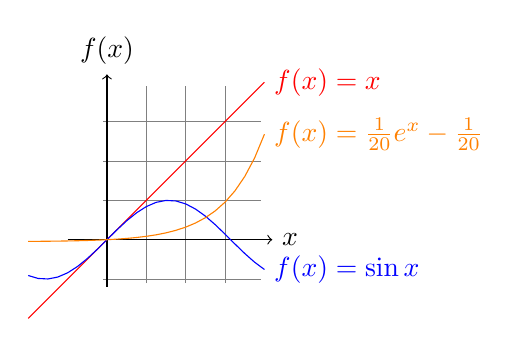
\begin{tikzpicture}[domain=-2:4, scale=0.5]
        \draw[very thin,color=gray] (-0.1,-1.1) grid (3.9,3.9);
        \draw[->] (-1,0) -- (4.2,0) node[right] {$x$};
        \draw[->] (0,-1.2) -- (0,4.2) node[above] {$f(x)$};
        \draw[color=red]    plot (\x,\x)             node[right] {$f(x) =x$};
        % \x r 表示弧度
        \draw[color=blue]   plot (\x,{sin(\x r)})    node[right] {$f(x) = \sin x$};
        \draw[color=orange] plot (\x,{0.05*exp(\x)-0.05}) node[right] {$f(x) = \frac{1}{20} e^x-\frac{1}{20}$};
    \end{tikzpicture}

\end{document}